\chapter{First chapter}

I am fake contents of the first chapter.

\section{First section}

I am the first section.

\begin{figure}
  \centering
  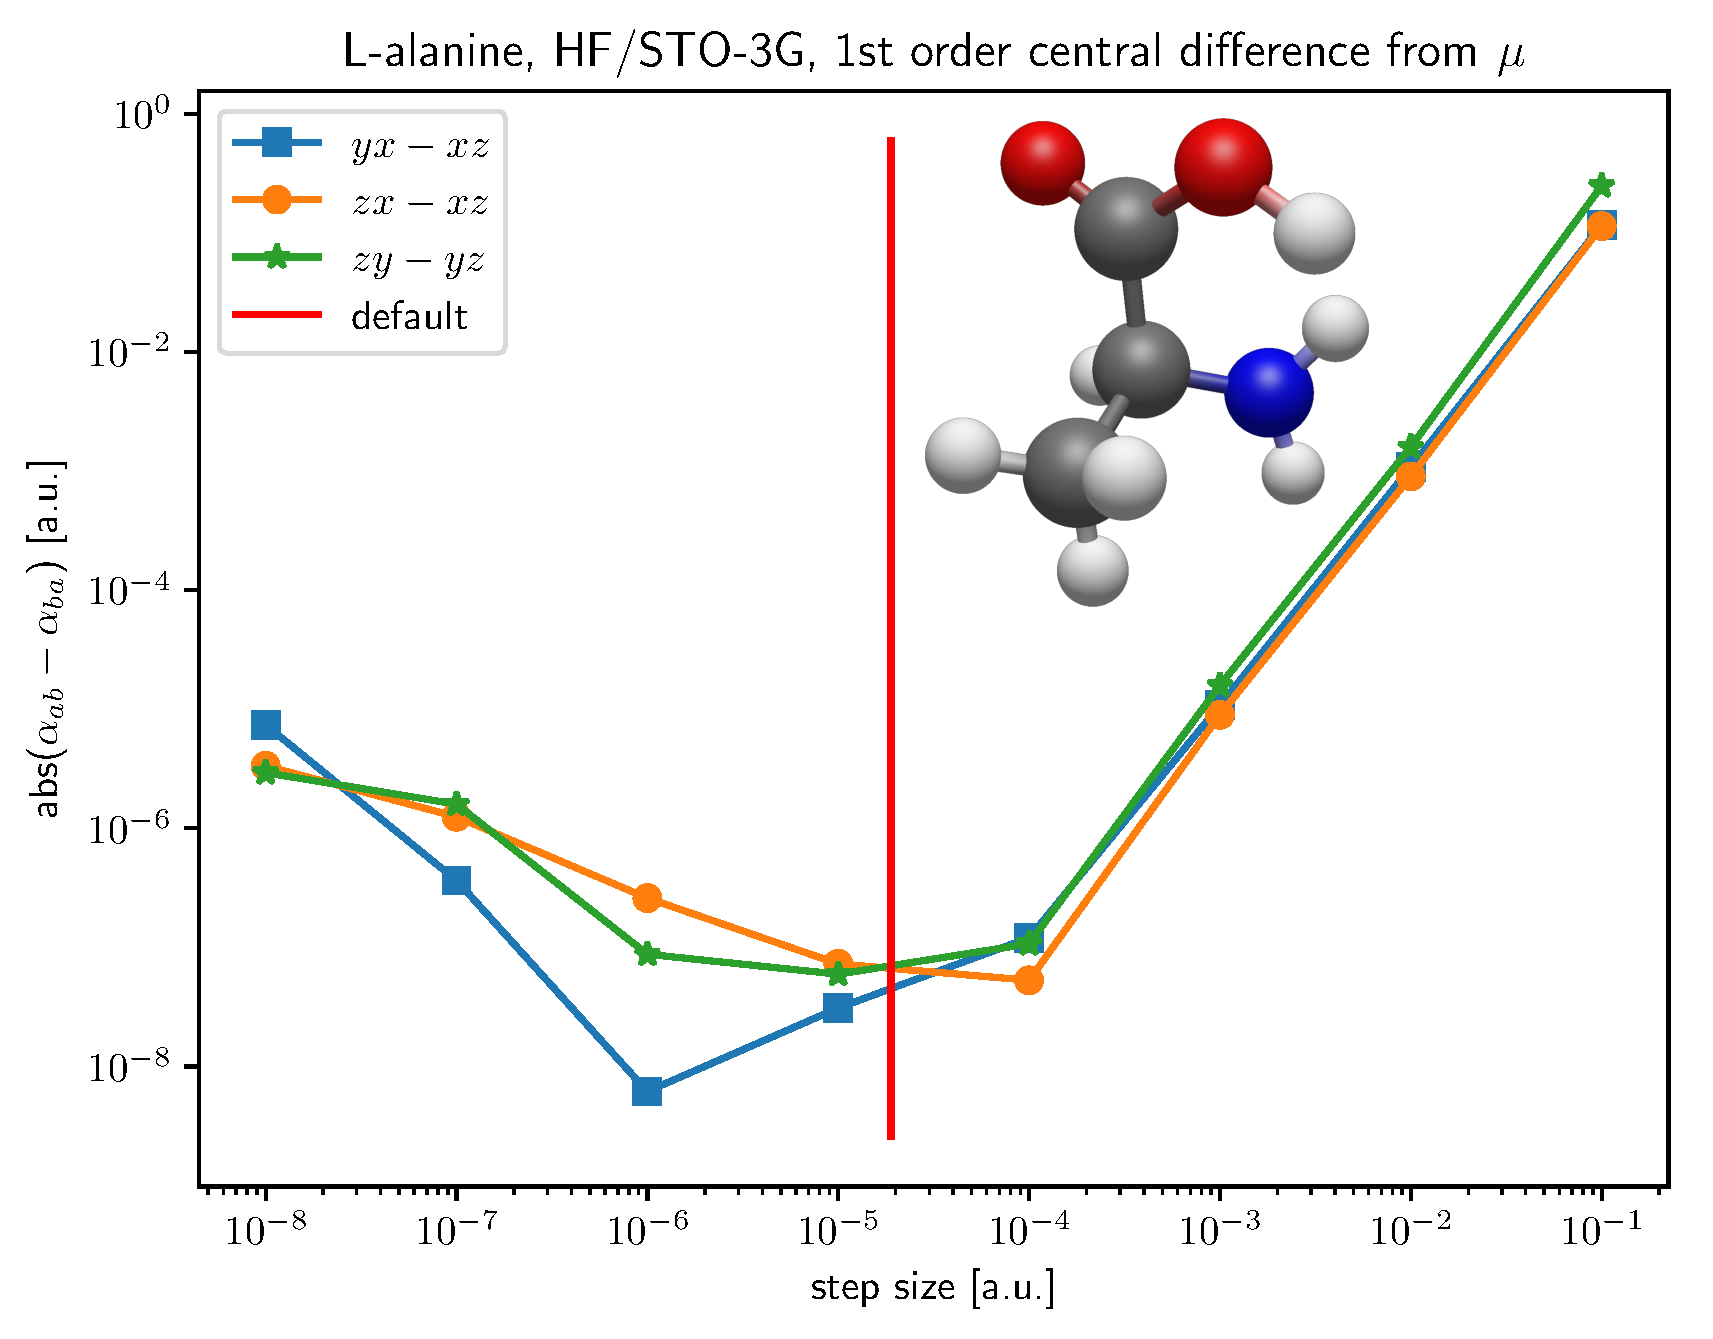
\includegraphics[width=\textwidth]{./diff_overlay.pdf}
  \caption{Asymmetry in the 1st-order finite-difference polarizability\label{fig:finite-difference-numerical-noise}}
\end{figure}

\begin{table}
  \centering
  \caption[MO coefficient derivatives and rotation matrices needed for energy derivatives]{Orders of MO coefficient derivatives and rotation matrices needed for energy derivatives following Wigner's \(2n+1\) rule. Reproduced from Ref.~\parencite{Yamaguchi1994}.}
  \label{tutorial:tab:wigner}
  \begin{tabular}{cccc}
    \toprule
    & CI: MO/CI space & MCSCF: MO/CI space & RHF: MO space \\
    \midrule
    Energy, \(E\) & \(C_{\mu}^{i}\), \(C_{I}\) & \(C_{\mu}^{i}\), \(C_{I}\) & \(C_{\mu}^{i}\) \\
    First Derivative, \(\frac{\partial E}{\partial a}\) & \(U^{a}\), \(C_{I}\) & \(C_{\mu}^{i}\), \(C_{I}\) & \(C_{\mu}^{i}\) \\
    Second Derivative, \(\frac{\partial^{2} E}{\partial a \partial b}\) & \(U^{ab}\), \(\frac{\partial C_{I}}{\partial a}\) & \(U^{a}\), \(\frac{\partial C_{I}}{\partial a}\) & \(U^{a}\) \\
    Third Derivative, \(\frac{\partial^{3} E}{\partial a \partial b \partial c}\) & \(U^{abc}\), \(\frac{\partial C_{I}}{\partial a}\) & \(U^{a}\), \(\frac{\partial C_{I}}{\partial a}\) & \(U^{a}\) \\
    Fourth Derivative, \(\frac{\partial^{4} E}{\partial a \partial b \partial c \partial d}\) & \(U^{abcd}\), \(\frac{\partial^{2} C_{I}}{\partial a \partial b}\) & \(U^{ab}\), \(\frac{\partial^{2} C_{I}}{\partial a \partial b}\) & \(U^{ab}\) \\
    Fifth Derivative, \(\frac{\partial^{5} E}{\partial a \partial b \partial c \partial d \partial e}\) & \(U^{abcde}\), \(\frac{\partial^{2} C_{I}}{\partial a \partial b}\) & \(U^{ab}\), \(\frac{\partial^{2} C_{I}}{\partial a \partial b}\) & \(U^{ab}\) \\
    \bottomrule
  \end{tabular}
\end{table}
